\documentclass[conference]{IEEEtran}
\usepackage{graphicx,booktabs,amsmath,amssymb,cite,url,array,multirow}
\usepackage[hidelinks]{hyperref}
\graphicspath{{figures/}}
\newcommand{\best}[1]{\textbf{#1}}
\begin{document}
\title{MarketPulse: Leakage-Controlled Market-Regime Classification and Regime-Change Probability Estimation with an HMM-Augmented, Calibrated Ensemble}
\author{\IEEEauthorblockN{[Author name(s)]}\IEEEauthorblockA{[Department, Institution], [email address]}}
\maketitle

\begin{abstract}
We study next-day classification of six market regimes (Bullish/Sideways/Bearish $\times$ Low/High volatility) and the probability that the regime label changes within 5, 10 or 20 trading days, using 7{,}302 real daily observations of the S\&P~500, VIX and Brent crude (1990--2018). The pipeline enforces chronological train/validation/test splits with an embargo, causal features, forward-filtered (not smoothed) hidden Markov model (HMM) states, walk-forward hyper-parameter search with Optuna, and validation-only calibration. A temperature-calibrated soft-voting ensemble over HMM-augmented features reaches a test log loss of 0.391 (95\% block-bootstrap CI 0.335--0.453), versus 0.783 for the persistence baseline, while persistence retains the best accuracy (0.861 vs.\ 0.843) and macro-F1 (0.837 vs.\ 0.800). Ablations show that the HMM state probabilities, 12 additional engineered features and cross-asset (VIX/Brent) covariates give no measurable test improvement, because the labels are deterministic functions of 60-day momentum and volatility (SHAP confirms these two features dominate). Error analysis shows 88\% of errors involve the trend dimension and error rates of 36\% for days closest to a label threshold versus 2.5\% for the farthest. The model is served by a FastAPI application in a Docker container. All code, tables and figures are reproducible from the repository.
\end{abstract}
\begin{IEEEkeywords}
market regimes, hidden Markov model, gradient boosting, probability calibration, Optuna, walk-forward validation, error analysis
\end{IEEEkeywords}

\section{Introduction}
Regime awareness---knowing whether markets are trending or range-bound, calm or turbulent---is central to risk management and asset allocation \cite{hamilton89,angbekaert02,kritzman12}. Two practical problems recur: (i) \emph{classify} the current/next regime, and (ii) \emph{estimate how likely a regime change is} over a short horizon. Published studies often evaluate on random splits, smooth HMM states with future data, or tune on the test period, all of which inflate results. This work builds a deliberately conservative pipeline and reports honest comparisons, including where simple baselines win.

\textbf{Contributions.} (1) A leakage-controlled pipeline (causal features, embargoed chronological splits, filtered HMM, validation-only calibration) with unit tests that perturb the future. (2) A feature-engineering and dimensionality-reduction study (33 causal features in 7 groups, PCA, t-SNE). (3) Optuna walk-forward tuning with a validation gate and experiment logging. (4) Benchmarks against re-implemented literature baselines with block-bootstrap confidence intervals, paired tests and a structured error analysis. (5) A containerised FastAPI inference service.

\section{Related Work and Baselines}
Hamilton's Markov-switching model \cite{hamilton89} and HMM inference \cite{rabiner89} underpin regime-switching asset-allocation work \cite{angbekaert02,kritzman12}. Volatility regimes are classically forecast with RiskMetrics EWMA \cite{riskmetrics96} and GARCH \cite{bollerslev86}; trend regimes with moving-average rules \cite{faber07}. Gradient-boosted trees \cite{chen16,ke17}, tuned by Bayesian optimisation \cite{akiba19}, are strong tabular learners, and temperature scaling \cite{guo17} is a simple post-hoc calibrator. SHAP \cite{lundberg17} provides attributions. We re-implement these \emph{method families} on a common task and split; we do not reproduce any paper's exact experiments and quote none of their numbers, as datasets, labels and horizons differ.

\section{Data}
\subsection{Dataset and Provenance}
The bundled dataset contains 7{,}302 trading days (2 Jan 1990--21 Dec 2018) of S\&P~500 OHLCV, the CBOE VIX close and Brent spot (USD/bbl). Sources are listed in the repository data card; the S\&P~500 series ends in Dec.\ 2018, so the test period excludes the 2020 and 2022 episodes. Cleaning removes duplicates, non-positive prices and $high<low$ rows (none occurred), forward-fills cross-asset gaps of at most five rows, and leaves 78 early Brent gaps missing (excluded by feature warm-up rather than imputed). Figure~\ref{fig:price} shows the series with regimes and VIX.

\begin{figure}[t]\centering\includegraphics[width=\columnwidth]{fig_price_regimes}
\caption{S\&P~500 coloured by rule-based regime, VIX below, shaded validation/test windows.}\label{fig:price}\end{figure}

\subsection{Regime Labels and Targets}
Trend is Bullish/Sideways/Bearish from the trailing 60-day return using the 30th/70th percentiles of the \emph{training} period (thresholds $-0.13\%$ and $+5.38\%$); volatility is High if 60-day annualised realised volatility exceeds the training median (12.5\%). This yields six classes. The supervised target is the label at $t{+}1$ given features at $t$. The transition target is $\mathbb{1}[\text{label changes within } h \text{ days}]$, $h\in\{5,10,20\}$, with 43\%, 60\% and 78\% prevalence on test.

\subsection{Splits}
Chronological 60/20/20 splits with a 20-row embargo: train 1990-10-15 to 2007-08-10 (4{,}241 rows), validation 2007-09-11 to 2013-04-04 (1{,}401), test 2013-05-03 to 2018-12-20 (1{,}420). Label thresholds, scaler, PCA, HMM, calibrators and tuning use training (or validation where stated) rows only.

\section{Feature Engineering and Dimensionality Reduction}
\subsection{Features}
Thirty-three causal features in seven groups: returns (5), volatility windows (4), momentum/RSI/drawdown (5), log-volume $z$-score (1), \emph{advanced volatility} (6: Parkinson and Garman--Klass range estimators, EWMA $\sigma$, vol-of-vol, skewness, kurtosis), \emph{trend} (6: SMA gaps, MACD histogram, Bollinger \%B, return autocorrelation, up-day ratio) and \emph{cross-asset} (6: VIX level, 5-day change, 60-day $z$-score, implied-minus-realised spread; Brent 20-day return and volatility, lagged one day for publication delay). A unit test corrupts all columns after row 3000 and asserts earlier features are unchanged. Figure~\ref{fig:corr} shows strong block structure (volatility estimators correlate $>0.9$).

\begin{figure}[t]\centering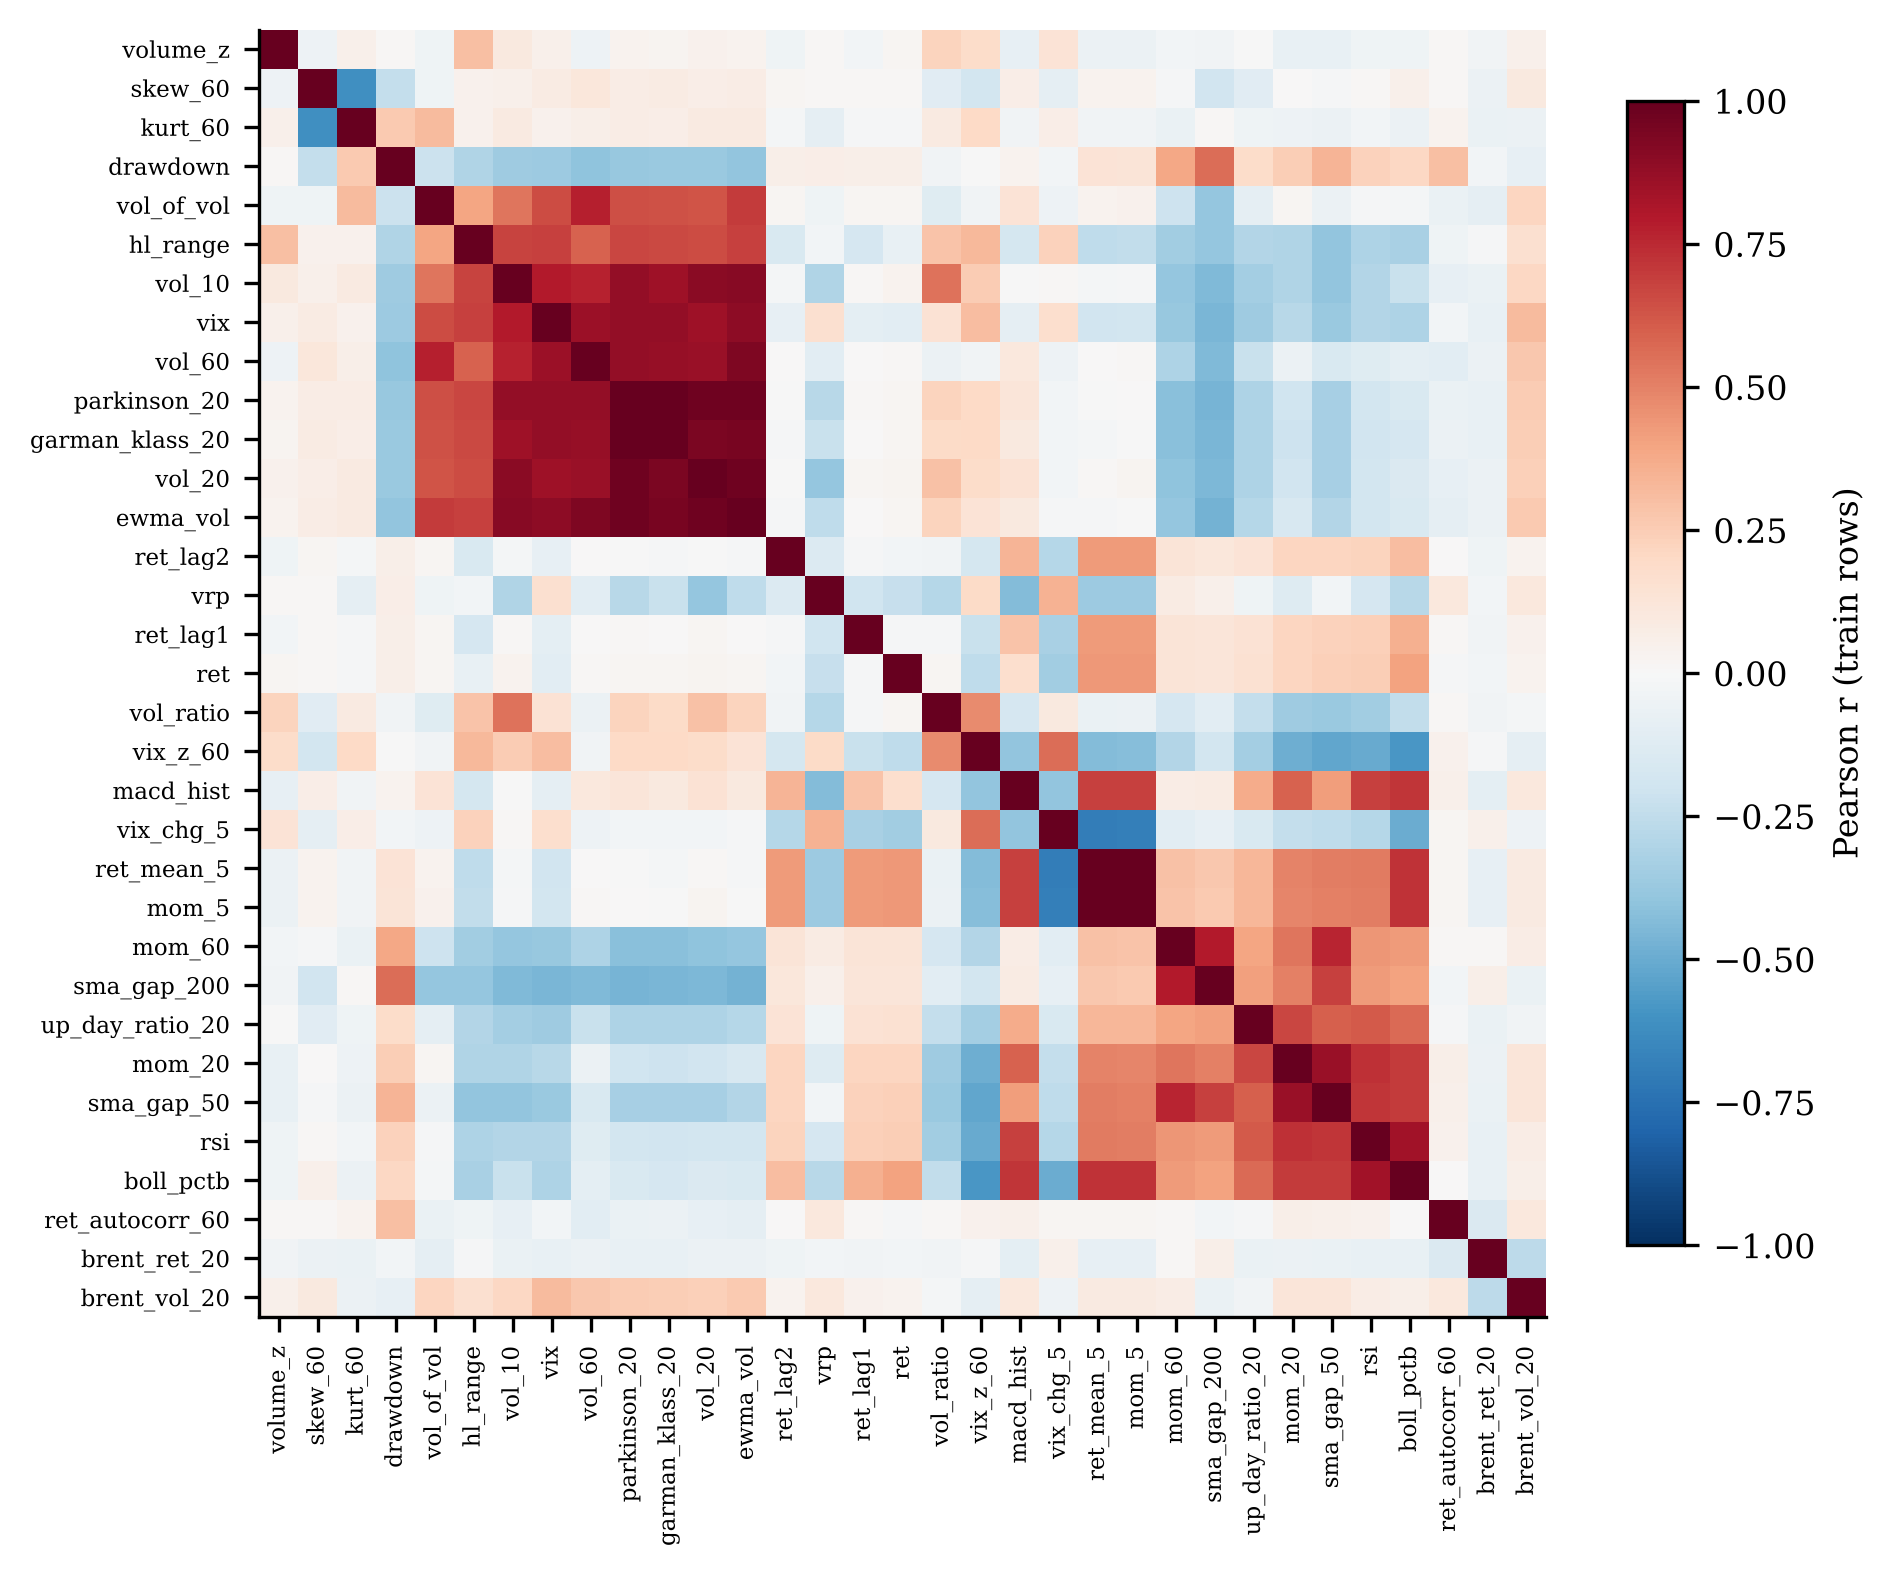
\includegraphics[width=.8\columnwidth]{fig_correlation}
\caption{Clustered feature correlation (training rows).}\label{fig:corr}\end{figure}

\subsection{PCA and t-SNE}
PCA on standardised, clipped training features needs 18 components for 95\% variance; PC1 (29.2\%) and PC2 (18.8\%) load on volatility estimators and short-term momentum, respectively (Fig.~\ref{fig:pca}). Regimes overlap heavily (silhouette $-0.03$), consistent with labels being threshold bands of continuous signals rather than natural clusters; t-SNE (Fig.~\ref{fig:tsne}) shows the same continuum with a distinct high-volatility arm. As model input, PCA hurts: logistic regression on 18 PCs scores macro-F1 0.697 versus 0.769 on raw features, and 3 PCs only 0.419 (Table~\ref{tab:pca}). Dimensionality reduction is therefore used for diagnosis, not prediction.

\begin{figure}[t]\centering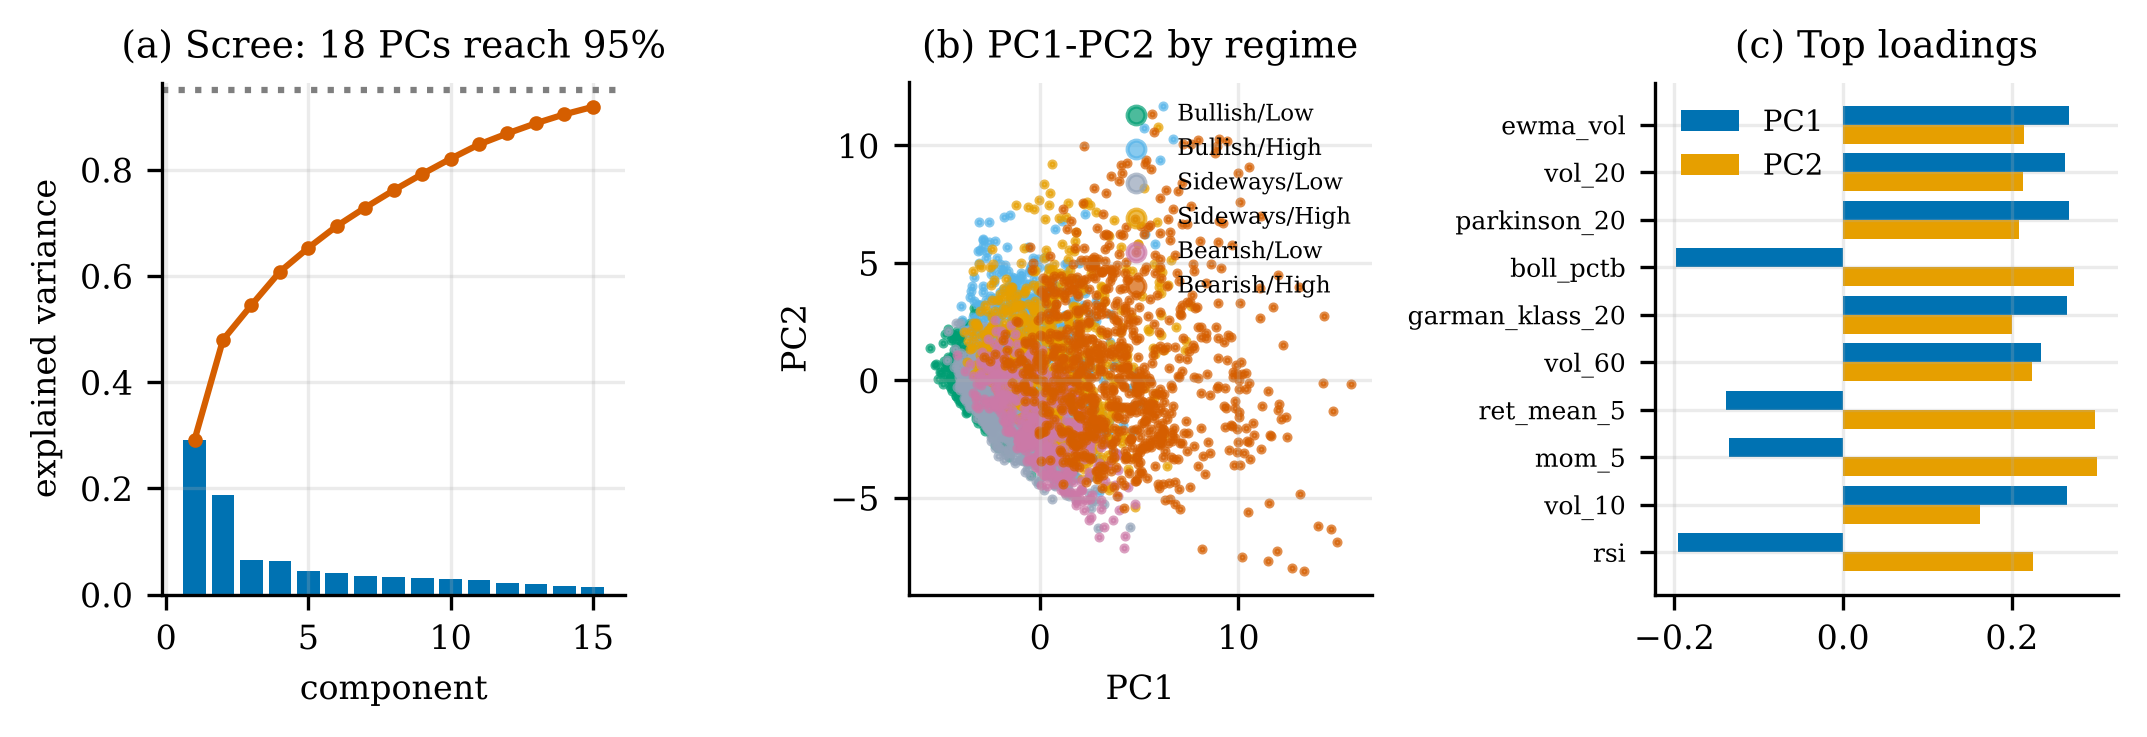
\includegraphics[width=\columnwidth]{fig_pca}
\caption{PCA: scree, PC1--PC2 by regime, loadings.}\label{fig:pca}\end{figure}
\begin{figure}[t]\centering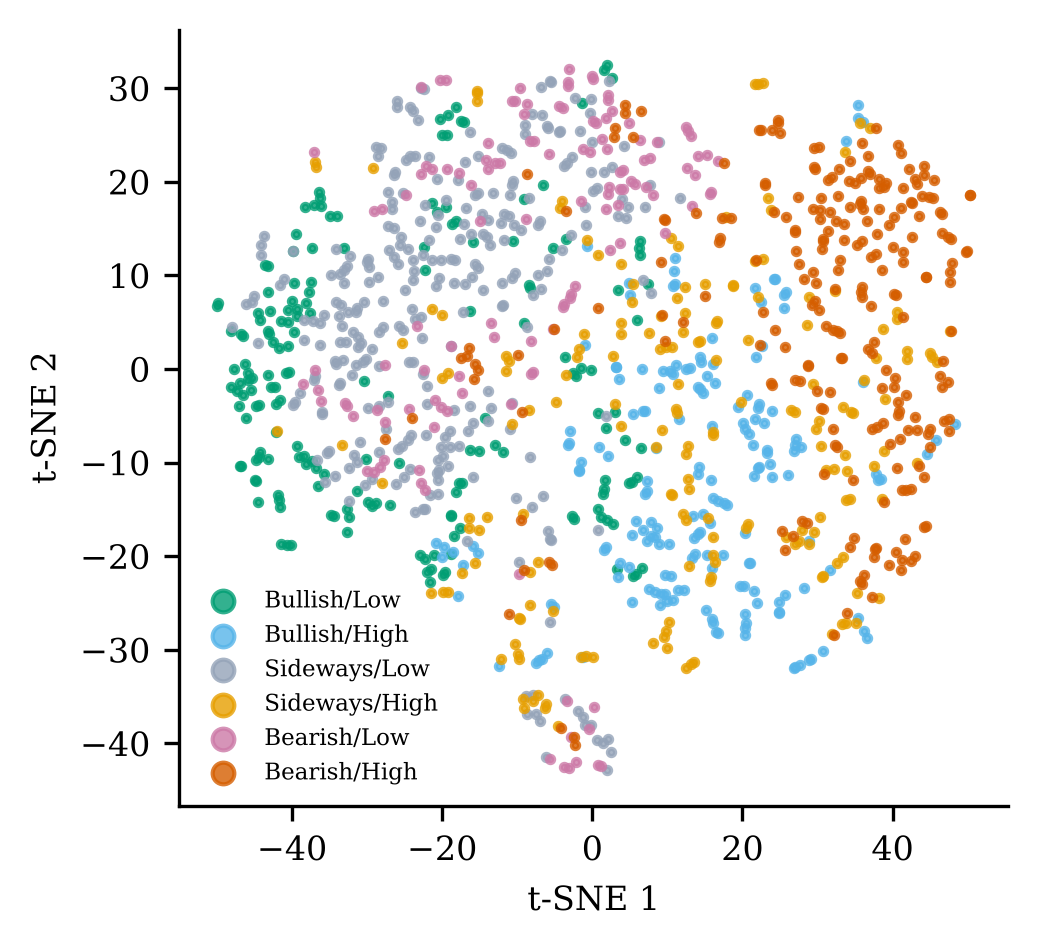
\includegraphics[width=.65\columnwidth]{fig_tsne}
\caption{t-SNE of training features (1{,}200-point subsample).}\label{fig:tsne}\end{figure}

\begin{table}[t]\caption{PCA input study (test, 6-class)}\label{tab:pca}\centering\small
\begin{tabular}{lcccc}\toprule Input & \#& Model & Macro-F1 & Log loss\\\midrule
PCA-3 & 3 & LR & 0.419 & 1.056\\ PCA-8 & 8 & LR & 0.602 & 0.722\\ PCA-18 (95\%) & 18 & LR & 0.697 & 0.625\\ PCA-18 (95\%) & 18 & LightGBM & 0.568 & 0.885\\ Raw features & 33 & LR & 0.769 & 0.438\\ Raw features & 33 & LightGBM & 0.782 & 0.543\\\bottomrule\end{tabular}\end{table}

\section{Methods}
\subsection{Filtered HMM}
A 3-state Gaussian HMM (full covariance, best of four EM restarts) is fitted on training rows over [return, 20-day volatility, 20-day momentum]. State probabilities are computed with the forward algorithm, $P(s_t\mid x_{1:t})$, plus the one-step predictive $P(s_{t+1}\mid x_{1:t})$; hmmlearn's smoothed posteriors are deliberately avoided because they use future observations. Test: truncating the series leaves earlier filtered probabilities identical (tolerance $10^{-9}$). State names (Bullish/Sideways/Bearish $\times$ volatility) are assigned from training-period state means by rank.

\subsection{Models}
Logistic regression, random forest, XGBoost and LightGBM are wrapped so probabilities always span all six classes. The \emph{soft-voting ensemble} averages member probabilities; the \emph{HMM-augmented ensemble} adds the six HMM columns; the \emph{calibrated hybrid} applies temperature scaling ($T=0.838$, fitted on validation log loss) \cite{guo17}. Transition models are LightGBM classifiers per horizon on features plus current regime and days-in-regime; calibration is chosen on validation among none/Platt/isotonic by forward-chained Brier score.

\subsection{Hyper-parameter Optimisation}
Optuna (TPE sampler, median pruner) \cite{akiba19} runs 25 trials per algorithm on training rows with 4 expanding-window folds separated by a 20-row gap, maximising negative log loss. Tuned parameters replace defaults only if validation log loss improves (a gate against over-fitting the search). Every study, parameter set and metric is appended to \texttt{experiments/runs.jsonl} with data fingerprint, library versions and seed.

\subsection{Statistical Protocol}
All headline numbers are on the untouched test split. Confidence intervals use a moving-block bootstrap (20-day blocks, 300 replicates); comparisons use paired block bootstrap of metric differences on identical resamples (500 replicates).

\section{Results}
\subsection{Hyper-parameter Tuning}
Optuna improved three of four algorithms on validation log loss (Fig.~\ref{fig:tune}): random forest 0.563$\to$0.369, XGBoost 0.383$\to$0.353, LightGBM 0.479$\to$0.367; logistic regression (0.371$\to$0.388) was rejected by the gate. For the hybrid, test log loss improved from 0.440 to 0.391 and macro-F1 from 0.783 to 0.800, with the 11--12 of 25 pruned trials per boosting study saving compute.

\begin{figure}[t]\centering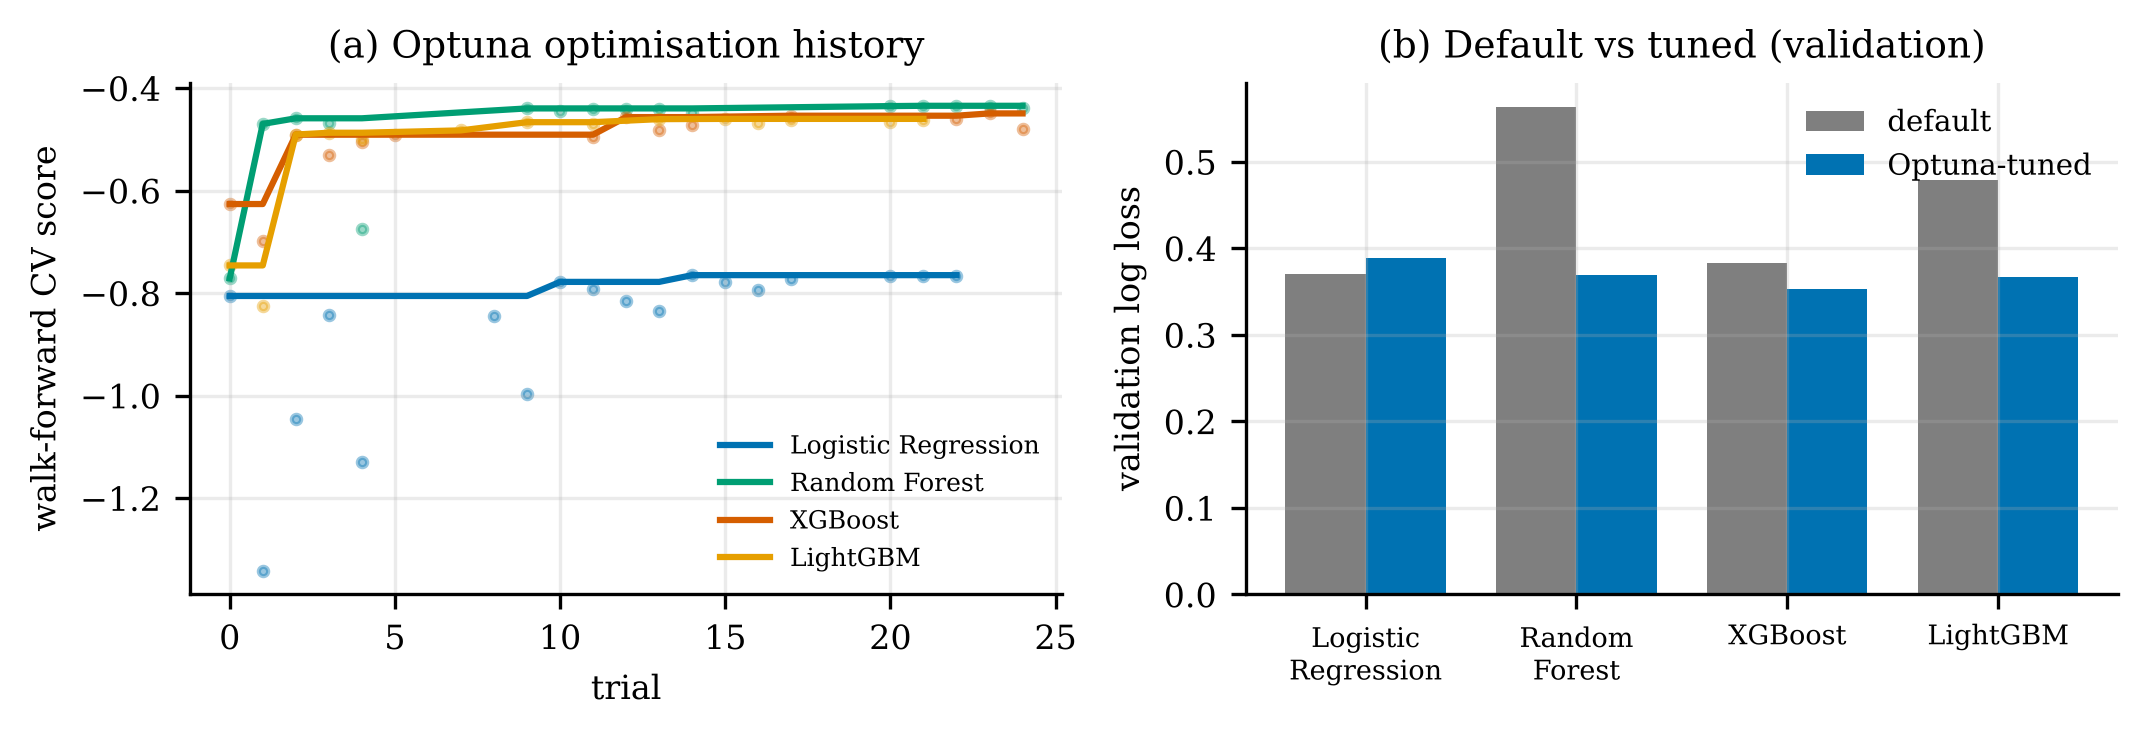
\includegraphics[width=\columnwidth]{fig_tuning}
\caption{Optuna history (best-so-far line) and default vs.\ tuned validation log loss.}\label{fig:tune}\end{figure}

\subsection{Six-class Benchmark}
Table~\ref{tab:main} and Fig.~\ref{fig:cmp} compare 12 methods. Three findings: (i) persistence has the best accuracy and macro-F1 because regimes last for weeks, but the worst-calibrated confidence (ECE 0.119, log loss 0.783); (ii) tuned tree models, the ensemble and the hybrid are statistically indistinguishable from one another on log loss (hybrid vs.\ XGBoost $\Delta=-0.004$, 95\% CI $[-0.016,0.012]$) yet significantly better than persistence ($\Delta=-0.395$, CI $[-0.496,-0.308]$), logistic regression ($-0.046$), LightGBM ($-0.026$) and MLP ($-0.052$); (iii) the standalone HMM-based classifier (macro-F1 0.268) cannot resolve six classes from three states, and PCA+LR loses 0.10 macro-F1. The hybrid has lower ECE (0.020) than the uncalibrated ensemble (0.031); temperature scaling gives a small but significant log-loss gain over the HMM-augmented ensemble ($\Delta=-0.008$, $p=0.024$).

\begin{table*}[t]\caption{Six-class next-day regime task on the test split (n = 1{,}420). 95\% block-bootstrap CIs in brackets.}\label{tab:main}\centering\small
\begin{tabular}{lccccc}\toprule Method & Accuracy & Macro-F1 & Log loss & Brier & ECE\\\midrule
Persistence baseline & \best{0.861} & \best{0.837} [0.790, 0.867] & 0.783 [0.655, 0.939] & 0.271 & 0.119\\
Soft-voting ensemble (tuned) & 0.847 & 0.808 [0.754, 0.837] & \best{0.391} [0.340, 0.446] & 0.216 & 0.031\\
\textbf{Calibrated hybrid (ours)} & 0.843 & 0.800 [0.750, 0.823] & \best{0.391} [0.335, 0.453] & 0.220 & \best{0.020}\\
XGBoost (tuned) & 0.849 & 0.815 [0.759, 0.846] & 0.395 [0.342, 0.452] & \best{0.214} & 0.021\\
HMM-augmented ensemble & 0.843 & 0.800 [0.750, 0.823] & 0.399 [0.348, 0.457] & 0.220 & 0.031\\
Random forest (tuned) & 0.856 & 0.825 [0.771, 0.858] & 0.410 [0.358, 0.465] & 0.216 & 0.038\\
LightGBM (tuned) & 0.837 & 0.798 [0.743, 0.827] & 0.416 [0.354, 0.484] & 0.231 & 0.034\\
Logistic regression & 0.820 & 0.769 [0.717, 0.802] & 0.438 [0.378, 0.507] & 0.254 & 0.016\\
MLP (64-32, $L_2$ tuned on val.) & 0.813 & 0.767 [0.707, 0.806] & 0.443 [0.378, 0.521] & 0.256 & 0.024\\
PCA (18) + logistic regression & 0.760 & 0.697 [0.629, 0.736] & 0.625 [0.520, 0.733] & 0.347 & 0.022\\
HMM-based (state$\to$next label) & 0.477 & 0.268 [0.218, 0.307] & 1.356 [1.221, 1.526] & 0.660 & 0.111\\
Majority class & 0.396 & 0.095 [0.081, 0.110] & 1.691 [1.652, 1.726] & 0.797 & 0.160\\\bottomrule\end{tabular}\end{table*}

\begin{figure}[t]\centering\includegraphics[width=\columnwidth]{fig_model_compare}
\caption{Test log loss and macro-F1 with 95\% block-bootstrap CIs; hybrid in orange.}\label{fig:cmp}\end{figure}

\subsection{Literature-method Baselines on Sub-tasks}
\textbf{Volatility regime} (binary, Table~\ref{tab:sub}): the hybrid collapsed to $P(\text{High})$ matches the 60-day realised-volatility score (log loss 0.053 each; ROC-AUC 0.999) and clearly beats GARCH(1,1)-$t$ (0.257), RiskMetrics EWMA (0.279) and VIX level (0.576) used as single predictors with Platt scaling fitted on train+validation. This is expected: the label \emph{is} thresholded 60-day volatility, so the 20-day-horizon forecasters carry less of the signal. \textbf{Trend regime} (3-class): persistence (macro-F1 0.864) $>$ ensemble (0.853) $>$ hybrid (0.851) $\gg$ SMA-50/200 rule (0.296). The rule scores poorly because it is not designed to reproduce a quantile-defined label; it is a reference point, not a fair rival.

\begin{table}[t]\caption{Sub-task benchmarks (test)}\label{tab:sub}\centering\small
\begin{tabular}{lccc}\toprule \multicolumn{4}{l}{\emph{Volatility regime (binary)}}\\ Method & Acc. & AUC & Log loss\\\midrule
Hybrid (collapsed) & 0.983 & 0.999 & \best{0.053}\\ Realised vol 60d & 0.988 & 0.998 & \best{0.053}\\ Persistence & 0.988 & 0.987 & 0.067\\ GARCH(1,1)-$t$ & 0.905 & 0.956 & 0.257\\ EWMA $\sigma$ & 0.895 & 0.948 & 0.279\\ VIX level & 0.752 & 0.834 & 0.576\\\midrule
\multicolumn{4}{l}{\emph{Trend regime (3-class)}}\\ Method & Acc. & \multicolumn{2}{c}{Macro-F1}\\\midrule
Persistence & 0.870 & \multicolumn{2}{c}{0.864}\\ Hybrid (collapsed) & 0.859 & \multicolumn{2}{c}{0.851}\\ HMM-based & 0.539 & \multicolumn{2}{c}{0.479}\\ SMA-50/200 rule & 0.287 & \multicolumn{2}{c}{0.296}\\\bottomrule\end{tabular}\end{table}

\subsection{Regime-change Probabilities}
On the harder transition task (Table~\ref{tab:trans}) LightGBM beats the constant, days-in-regime hazard, logistic regression and HMM-implied baselines in PR-AUC at 5 and 10 days; at 5 days PR-AUC is 0.636 [0.550, 0.728] versus 0.427 prevalence, but intervals overlap with the empirical hazard (0.591), so the evidence of superiority is weak at this sample size. Validation-selected calibration chose ``none'' for all horizons; the post-hoc study agrees: Platt and isotonic calibrators fitted on the 2007--2013 validation window \emph{worsen} test Brier (e.g.\ 10-day: 0.223 none, 0.228 Platt, 0.235 isotonic) because the validation window had different change frequencies. Calibrating on a window unlike deployment can hurt.

\begin{table}[t]\caption{Regime change within $h$ days (test; PR-AUC [95\% CI])}\label{tab:trans}\centering\small
\begin{tabular}{lccc}\toprule Method & $h{=}5$ & $h{=}10$ & $h{=}20$\\\midrule
Prevalence & 0.427 & 0.595 & 0.776\\ Days-in-regime hazard & 0.591 & 0.728 & 0.846\\ HMM-implied & 0.476 & 0.636 & 0.802\\ Logistic regression & 0.570 & 0.748 & \best{0.895}\\ LightGBM (ours) & \best{0.636} & \best{0.767} & 0.886\\\bottomrule\end{tabular}\end{table}

\subsection{Ablations}
\emph{Feature groups} (single LightGBM, test macro-F1, Fig.~\ref{fig:abl}): returns only 0.269; $+$volatility 0.409; $+$momentum 0.783; $+$volume 0.787; $+$advanced volatility 0.778; $+$trend 0.776; $+$cross-asset 0.782. Momentum is decisive; later groups add nothing within noise. For the transition task the extra groups were slightly \emph{harmful} (5-day PR-AUC 0.671 core, 0.652 with advanced, 0.637 full; 3 seeds, sd $\le0.008$). \emph{HMM information}: ensemble without HMM columns: log loss 0.391 vs.\ 0.399 with them (test). SHAP (Fig.~\ref{fig:shap}) explains why: \texttt{mom\_60} and \texttt{vol\_60}, which define the labels, carry nearly all attribution (mean $|$SHAP$|$ 1.26 and 1.22 versus $\le0.13$ for any other feature). We keep the extended features and HMM in the shipped model as documented, evidence-backed non-contributors rather than tuning the feature set on the test split.

\begin{figure}[t]\centering\includegraphics[width=\columnwidth]{fig_feature_ablation}
\caption{Cumulative feature-group ablation (test).}\label{fig:abl}\end{figure}
\begin{figure}[t]\centering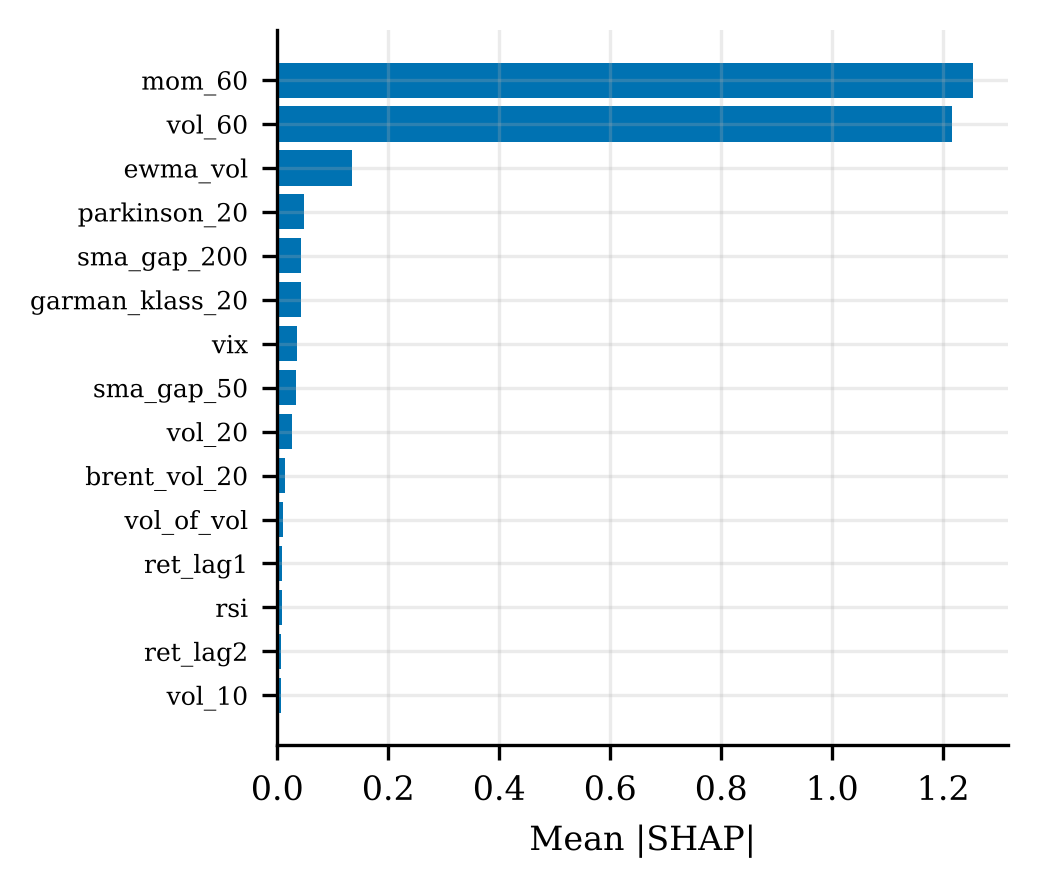
\includegraphics[width=.62\columnwidth]{fig_shap}
\caption{Mean $|$SHAP$|$, tuned XGBoost, 400 test rows.}\label{fig:shap}\end{figure}

\subsection{Calibration}
Fig.~\ref{fig:rel} shows top-class reliability: the hybrid's confidence tracks accuracy within about 0.05--0.10 for bins above 0.6 (error 4.3\% at confidence $>0.9$ with 805 days, 52\% for confidence 0.5--0.6) while persistence's implicit 98\% confidence is right only 86\% of the time.

\begin{figure}[t]\centering\includegraphics[width=\columnwidth]{fig_reliability}
\caption{Reliability of regime probabilities and transition probabilities (test).}\label{fig:rel}\end{figure}

\section{Error Analysis}
Analysis is on the 1{,}420 test days (hybrid error 15.7\%, persistence 13.9\%).
\begin{itemize}
\item \textbf{Which dimension:} 88\% of errors are trend-only, 10\% volatility-only, 2\% both. Volatility regimes are nearly deterministic; the trend band is where the model errs.
\item \textbf{Threshold proximity:} error rate is 36.3\% for the quartile of days closest to a trend/volatility threshold and 2.5\% for the farthest quartile (Fig.~\ref{fig:err}a). Most errors are unavoidable coin-flips about which side of an arbitrary cut-off tomorrow's 60-day return lands on.
\item \textbf{Change days:} of 197 true regime changes, the hybrid flags 80 and catches 28 (recall 14\%, precision 35\%); on non-change days it is 95.7\% accurate, versus 100\%/0\% for persistence. The model's net advantage is probabilistic quality, not change detection.
\item \textbf{Confusions:} Sideways/Low$\to$Bullish/Low (47 days, 21\% of errors) and the reverse dominate; Bullish/High has the lowest recall (0.50, $n=86$), and Bullish/High $\to$ Sideways/High is the main leak.
\item \textbf{Environment and time:} errors are highest in mid-VIX regimes (20.0\%) and lowest at VIX $>20.6$ (7.9\%); by year the hybrid is worse than persistence in 2013--2016 (peak 22.2\% in 2016, the Aug-2015/Jan-2016 sell-offs) and better in 2018 (13.1\% vs 15.5\%) (Fig.~\ref{fig:err}c).
\item \textbf{Overconfident errors:} the ten most confident mistakes (0.95--0.98) are mostly Bearish/Low days predicted as Sideways/Low in 2013--2018, e.g.\ 2014-09-24 and 2016-06-23 (the Brexit vote): abrupt moves that push the 60-day return across the bearish cut-off.
\end{itemize}
\begin{figure}[t]\centering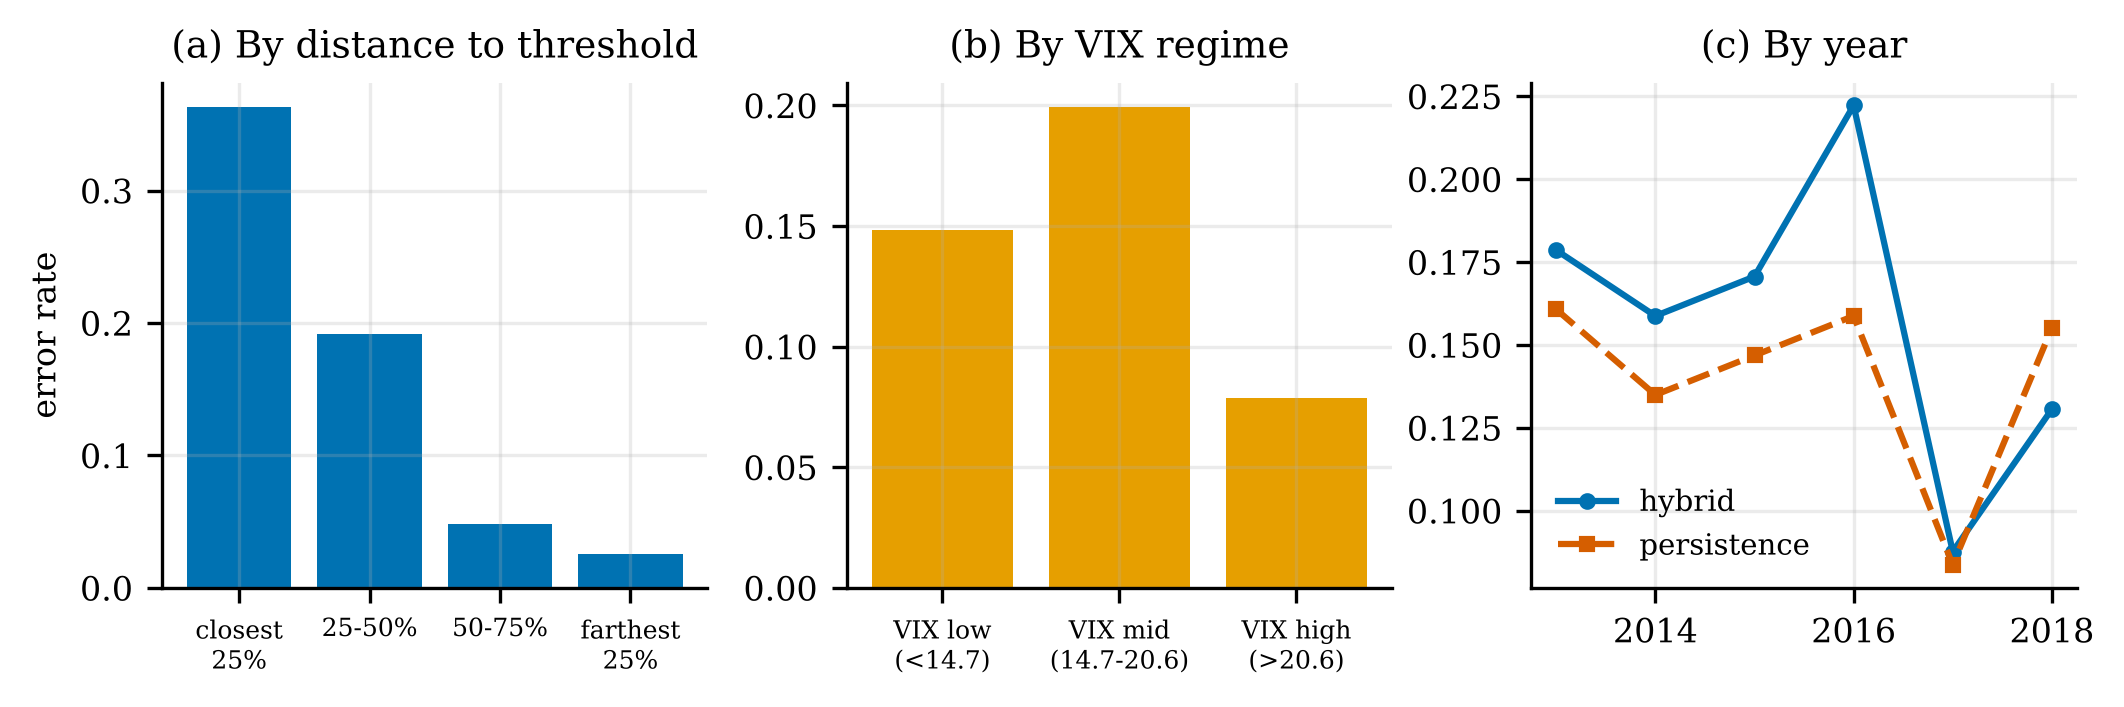
\includegraphics[width=\columnwidth]{fig_errors}
\caption{Error rate by distance to threshold, VIX regime and year.}\label{fig:err}\end{figure}
\begin{figure}[t]\centering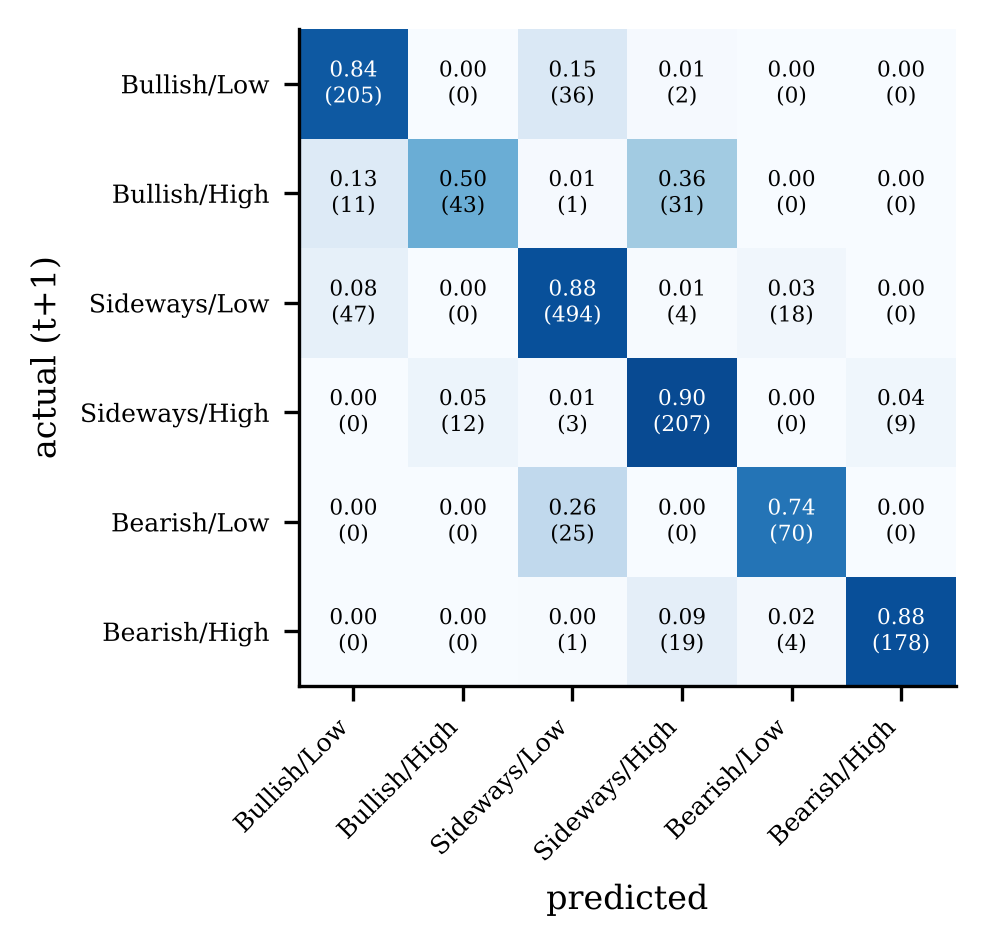
\includegraphics[width=.7\columnwidth]{fig_confusion}
\caption{Row-normalised confusion matrix of the hybrid (counts in brackets).}\label{fig:conf}\end{figure}

\section{System and Deployment}
\textbf{Application.} A FastAPI service (\texttt{api/main.py}) loads a 5\,MB model bundle (calibrated ensemble, HMM, label thresholds, transition models and calibrators) and exposes \texttt{GET /health}, \texttt{/model}, \texttt{/demo}, \texttt{POST /predict} (validated OHLCV+VIX+Brent history, $\ge$320 rows) and a browser demo page. Responses give the current regime and its age, next-day class probabilities, a low-confidence flag, regime-change probabilities at 5/10/20 days, and flag whether the as-of date lies in the training or validation window. Tests verify that API outputs equal the training pipeline's outputs to $2\times10^{-4}$ and that malformed input (short history, $high<low$, missing VIX, unsorted dates) returns HTTP 422. A Streamlit dashboard (nine pages, including Feature Lab and Benchmarks \& Errors) supports exploration.
\textbf{Containerisation.} A \texttt{python:3.13-slim} Dockerfile installs pinned runtime dependencies, runs as non-root (uid 1000), listens on \texttt{\$PORT} (7860, Hugging Face Spaces), and defines a health check; \texttt{docker-compose.yml} adds the dashboard as an optional service. Deployment steps for Hugging Face Spaces (Docker SDK) and AWS App Runner are in \texttt{docs/DEPLOYMENT.md}. Live URL: [insert after deployment].
\textbf{Reproducibility.} \texttt{python train.py --tune} regenerates every table, figure and the bundle (about 17 minutes on 2 CPU cores); 30 automated tests cover causality, splits, calibration, tuning, tracking, benchmarks, errors and the API.

\section{Limitations and Ethics}
(i) Labels are rule-based, so supervised accuracy largely measures persistence and threshold proximity; the task is not tradable alpha. (ii) One instrument and one test window (2013--2018, a low-volatility bull market with few crises); results may not transfer to 2020 or 2022. (iii) Bootstrap CIs account for serial dependence but not label-threshold or model-selection uncertainty. (iv) Baselines are method-family re-implementations with modest tuning, not paper replications. (v) The S\&P~500 file's redistribution licence is unstated. (vi) The system is an educational tool; it gives no investment advice and no trading signal.

\section{Conclusion}
A carefully leakage-controlled pipeline shows that calibrated tree ensembles substantially improve the probabilistic quality of regime forecasts over persistence (log loss 0.391 vs.\ 0.783) while persistence remains hard to beat on hard-label accuracy. HMM states, advanced features and cross-asset covariates did not help on these labels---a negative result we report instead of tuning around. Future work: market-defined (not threshold-defined) regime targets, additional instruments and post-2018 data, and economic-value evaluation with transaction costs.

\begin{thebibliography}{99}\small
\bibitem{hamilton89} J. D. Hamilton, ``A new approach to the economic analysis of nonstationary time series and the business cycle,'' \emph{Econometrica}, vol. 57, no. 2, pp. 357--384, 1989.
\bibitem{rabiner89} L. R. Rabiner, ``A tutorial on hidden Markov models and selected applications in speech recognition,'' \emph{Proc. IEEE}, vol. 77, no. 2, pp. 257--286, 1989.
\bibitem{angbekaert02} A. Ang and G. Bekaert, ``International asset allocation with regime shifts,'' \emph{Rev. Financial Studies}, vol. 15, no. 4, pp. 1137--1187, 2002.
\bibitem{kritzman12} M. Kritzman, S. Page, and D. Turkington, ``Regime shifts: Implications for dynamic strategies,'' \emph{Financial Analysts J.}, vol. 68, no. 3, pp. 22--39, 2012.
\bibitem{riskmetrics96} J.P. Morgan/Reuters, \emph{RiskMetrics---Technical Document}, 4th ed., 1996.
\bibitem{bollerslev86} T. Bollerslev, ``Generalized autoregressive conditional heteroskedasticity,'' \emph{J. Econometrics}, vol. 31, no. 3, pp. 307--327, 1986.
\bibitem{faber07} M. T. Faber, ``A quantitative approach to tactical asset allocation,'' \emph{J. Wealth Management}, vol. 9, no. 4, pp. 69--79, 2007.
\bibitem{chen16} T. Chen and C. Guestrin, ``XGBoost: A scalable tree boosting system,'' in \emph{Proc. KDD}, 2016, pp. 785--794.
\bibitem{ke17} G. Ke \emph{et al.}, ``LightGBM: A highly efficient gradient boosting decision tree,'' in \emph{Proc. NeurIPS}, 2017.
\bibitem{akiba19} T. Akiba \emph{et al.}, ``Optuna: A next-generation hyperparameter optimization framework,'' in \emph{Proc. KDD}, 2019, pp. 2623--2631.
\bibitem{guo17} C. Guo, G. Pleiss, Y. Sun, and K. Q. Weinberger, ``On calibration of modern neural networks,'' in \emph{Proc. ICML}, 2017, pp. 1321--1330.
\bibitem{lundberg17} S. M. Lundberg and S.-I. Lee, ``A unified approach to interpreting model predictions,'' in \emph{Proc. NeurIPS}, 2017.
\end{thebibliography}
\end{document}
